\renewcommand{\chapterlabel}{Appendix}
\chapter{OPESN sub-reservoir connections}
\label{app:sub_reservoir_connections}

\subsection{OPESN with stochastic connections}

Here I will explain the implementation of the OPESN with one-to-one sub-reservoir connections that are stochastically activated constant value connections. At every time step each partition chooses exactly one destination partition according to the ordinal transition probabilities. Firstly we will define a stochastic function $F_{i}(t)$ which selects a destination partition $j$ for each partition $i$ at each time step (t) such that
\[
    P[F_{i}(t) = j] = p_{i,j}
\]
where $F_{i}(t) \in [1, ..., N_{obs}]$. Then we can define each submatrix $\mathbf{W}_{i,j}$ in the recurrence matrix $\mathbf{W}_{rec}$ as we did for other connection methods in Chapter \ref{chap:OPESNs}:
\[
\mathbf{W}_{i,j}(t) =
\begin{cases}
\mathbf{W}_{ER_{i,j}}, & i = j, \\
c\mathbf{I}, & i \neq j \text{ and } F_{i}(t) = j, \\
\mathbf{0}, & \text{otherwise}.
\end{cases}
\]
Practically, this involves instantiating the constant one-to-one connections solution
\[
\mathbf{W}_{i,j} =
\begin{cases}
\mathbf{W}_{ER_{i,j}}, & i = j, \\
c\mathbf{I}, & i \neq j \text{ and } p_{i,j} > 0, \\
\mathbf{0}, & \text{otherwise},
\end{cases}
\]
and masking each $\mathbf{W}_{i,j}$ at each time step if $F_{i}(t) \neq j$ by setting $\mathbf{W}_{i,j} = \mathbf{0}$. This masking process makes the evolution of the reservoir extremely inefficient, so it is necessary to cache the possible masked states of the resevoir for each combination of stochastically selected partitions. The stochastic OPESN with $m=4$ has $(4!)(4!)=576$ possible combinations of partitions, which creates a memory usage problem for storing the cached masked states of the reservoir. Thus we cached the most common combinations and allowed the remaining to be computed at each time step, including a partition transition pair in the most common combinations according to a transition probability threshold.


\pagebreak

\subsection{Further sub-reservoir connection experiments}

\begin{figure}[h]
    \centering
    % ensure the graphic is centered and scaled to the text width without overflow
    \makebox[\textwidth][c]{%
        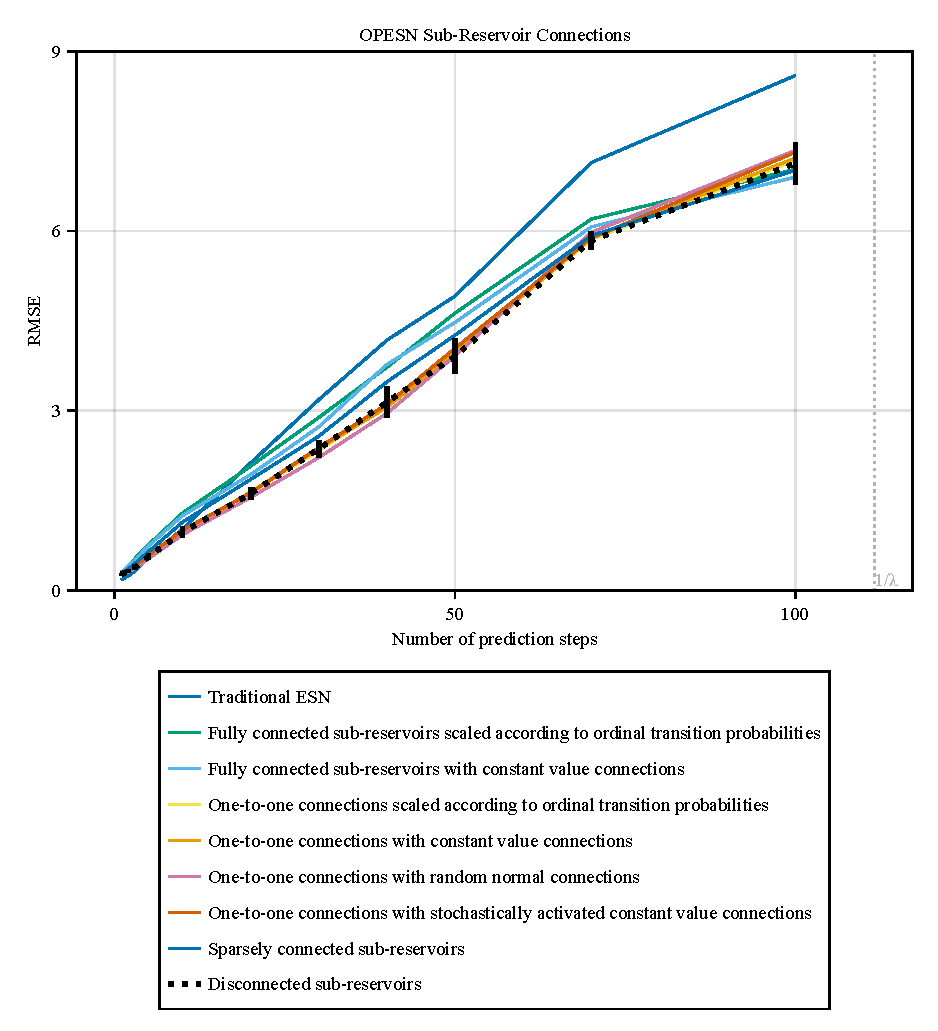
\includegraphics{../Images/OPESN/OPESN_recursive_sub_reservoir_connections_m=3.pdf}%[width=1.2\textwidth]
    }%[width=\textwidth,keepaspectratio]
    \caption{Recursive prediction RMSE for the OPESN for all variants of sub-reservoir connections. Delay $\tau=20$, $m=3$, noise level $\alpha=0.1$, and total reservoir size $k=468$.}
    \label{fig:OPESN_recursive_sub_reservoir_connections_m_2}
\end{figure}

\begin{figure}[h]
    \centering
    % ensure the graphic is centered and scaled to the text width without overflow
    \makebox[\textwidth][c]{%
        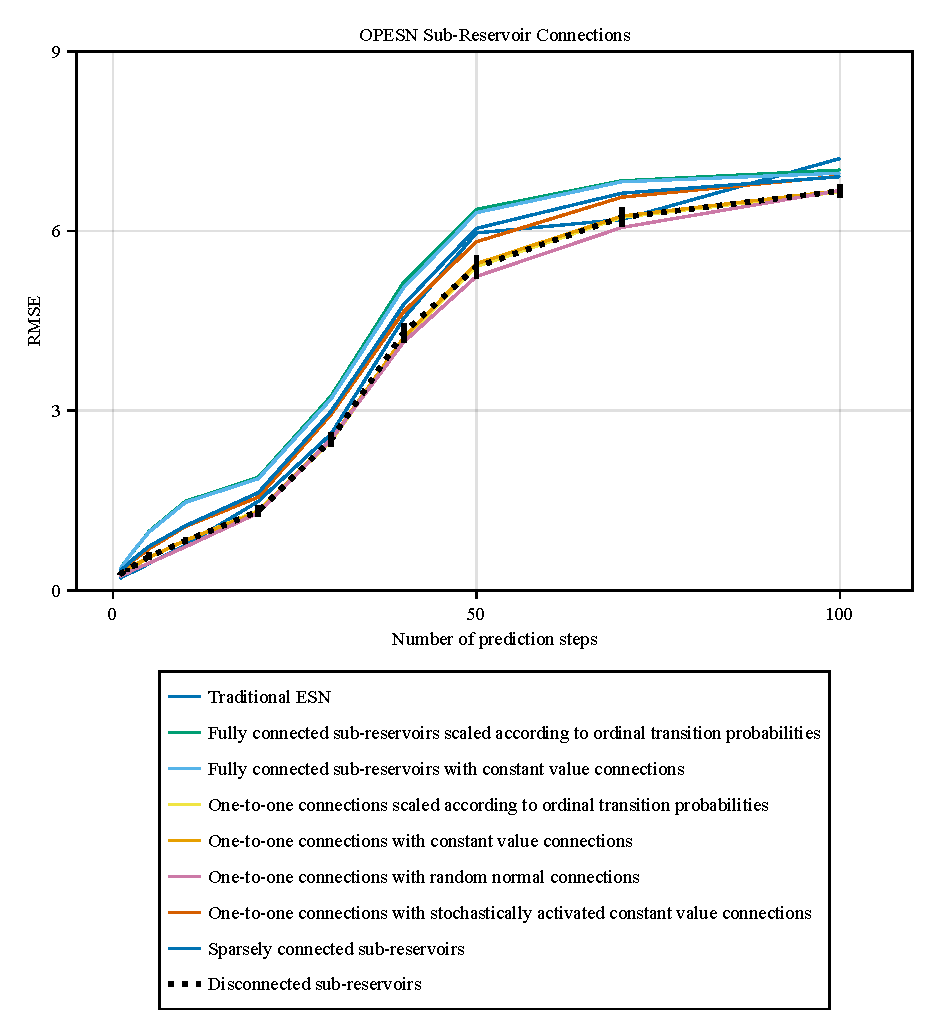
\includegraphics{../Images/OPESN/OPESN_direct_sub_reservoir_connections_m=4.pdf}%[width=1.2\textwidth]
    }%[width=\textwidth,keepaspectratio]
    \caption{Direct prediction RMSE for the OPESN for all variants of sub-reservoir connections. Delay $\tau=20$, $m=4$, noise level $\alpha=0.1$, and total reservoir size $k=468$.}
    \label{fig:OPESN_direct_sub_reservoir_connections_m_2}
\end{figure}

\begin{figure}[h]
    \centering
    % ensure the graphic is centered and scaled to the text width without overflow
    \makebox[\textwidth][c]{%
        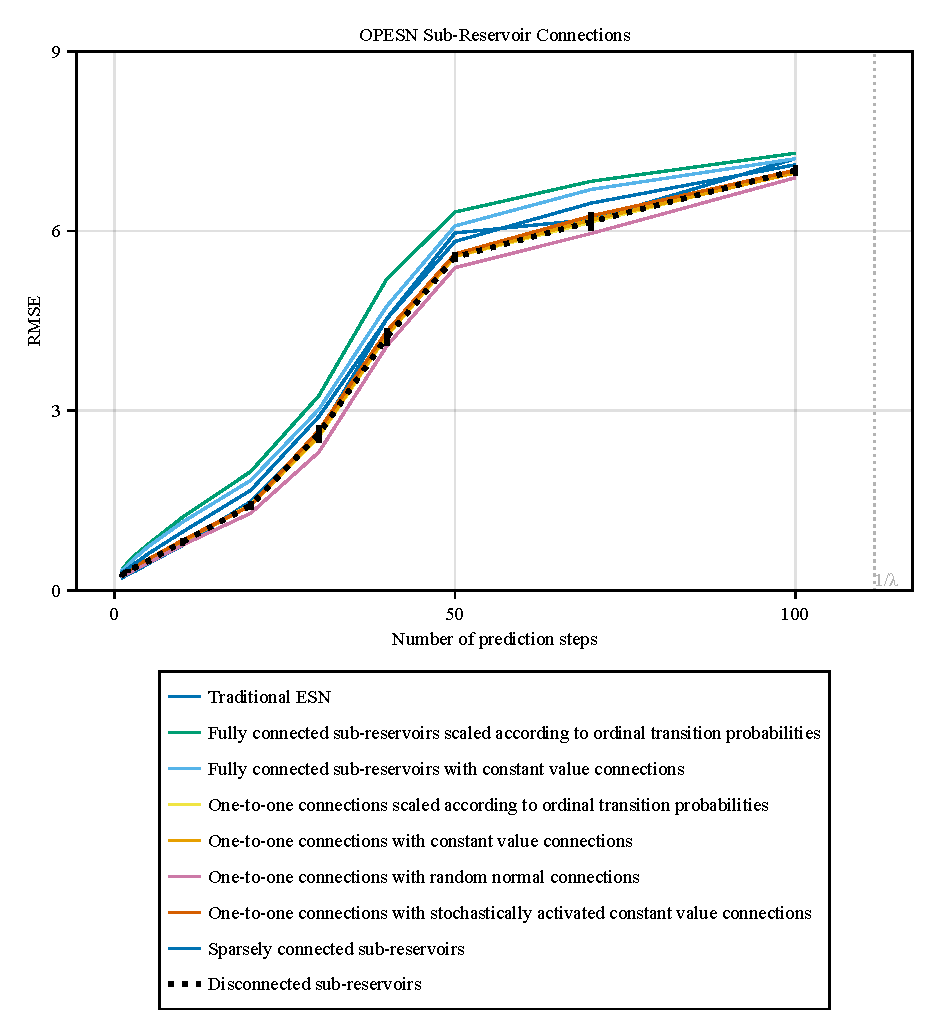
\includegraphics{../Images/OPESN/OPESN_direct_sub_reservoir_connections_m=3.pdf}%[width=1.2\textwidth]
    }%[width=\textwidth,keepaspectratio]
    \caption{Direct prediction RMSE for the OPESN for all variants of sub-reservoir connections. Delay $\tau=20$, $m=3$, noise level $\alpha=0.1$, and total reservoir size $k=468$.}
    \label{fig:OPESN_direct_sub_reservoir_connections_m_3}
\end{figure}